%!TEX root = ../TTK4900-MHT.tex

\chapter{Theoretical Background}\label{chapter:theoretical_background}
\section{Radar}
\subsection{Overview}
\gls{radar_acr} is a detection technology that uses radio waves to observe stationary and moving objects. A transmitter sends out radio waves and a receiver is waiting for reflected echo's from objects, were the time the echo is delayed determines the distance to the object. The transmitter and receiver will in many situations be in the same location, and can be both stationary or mobile and have fixed or rotating orientation. Depending on frequency, a radar can observe solid objects like aircraft, ships, terrain, road vehicles and less solid objects like people and weather formations.
\begin{figure}
\centering
\begin{minipage}{0.3\textwidth}
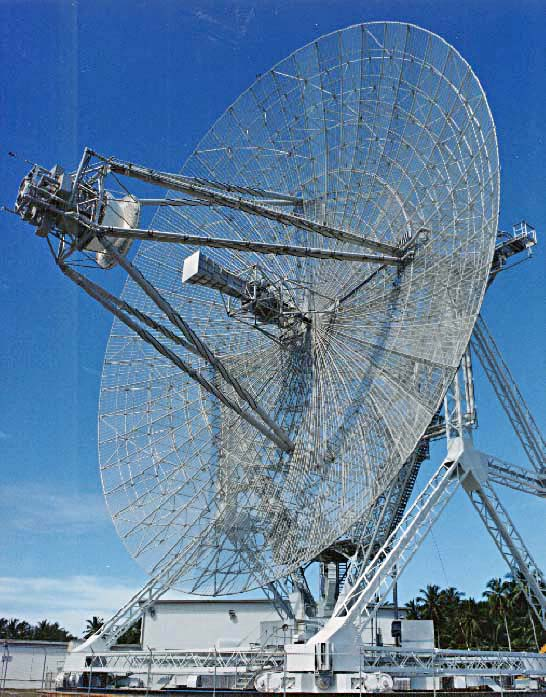
\includegraphics[width=0.9\textwidth]{Fixed_radar_antenna}
\caption{Fixed radar antenna}\label{fig:fixed_radar_antenna}
\end{minipage}\hfill
\begin{minipage}{0.3\textwidth}
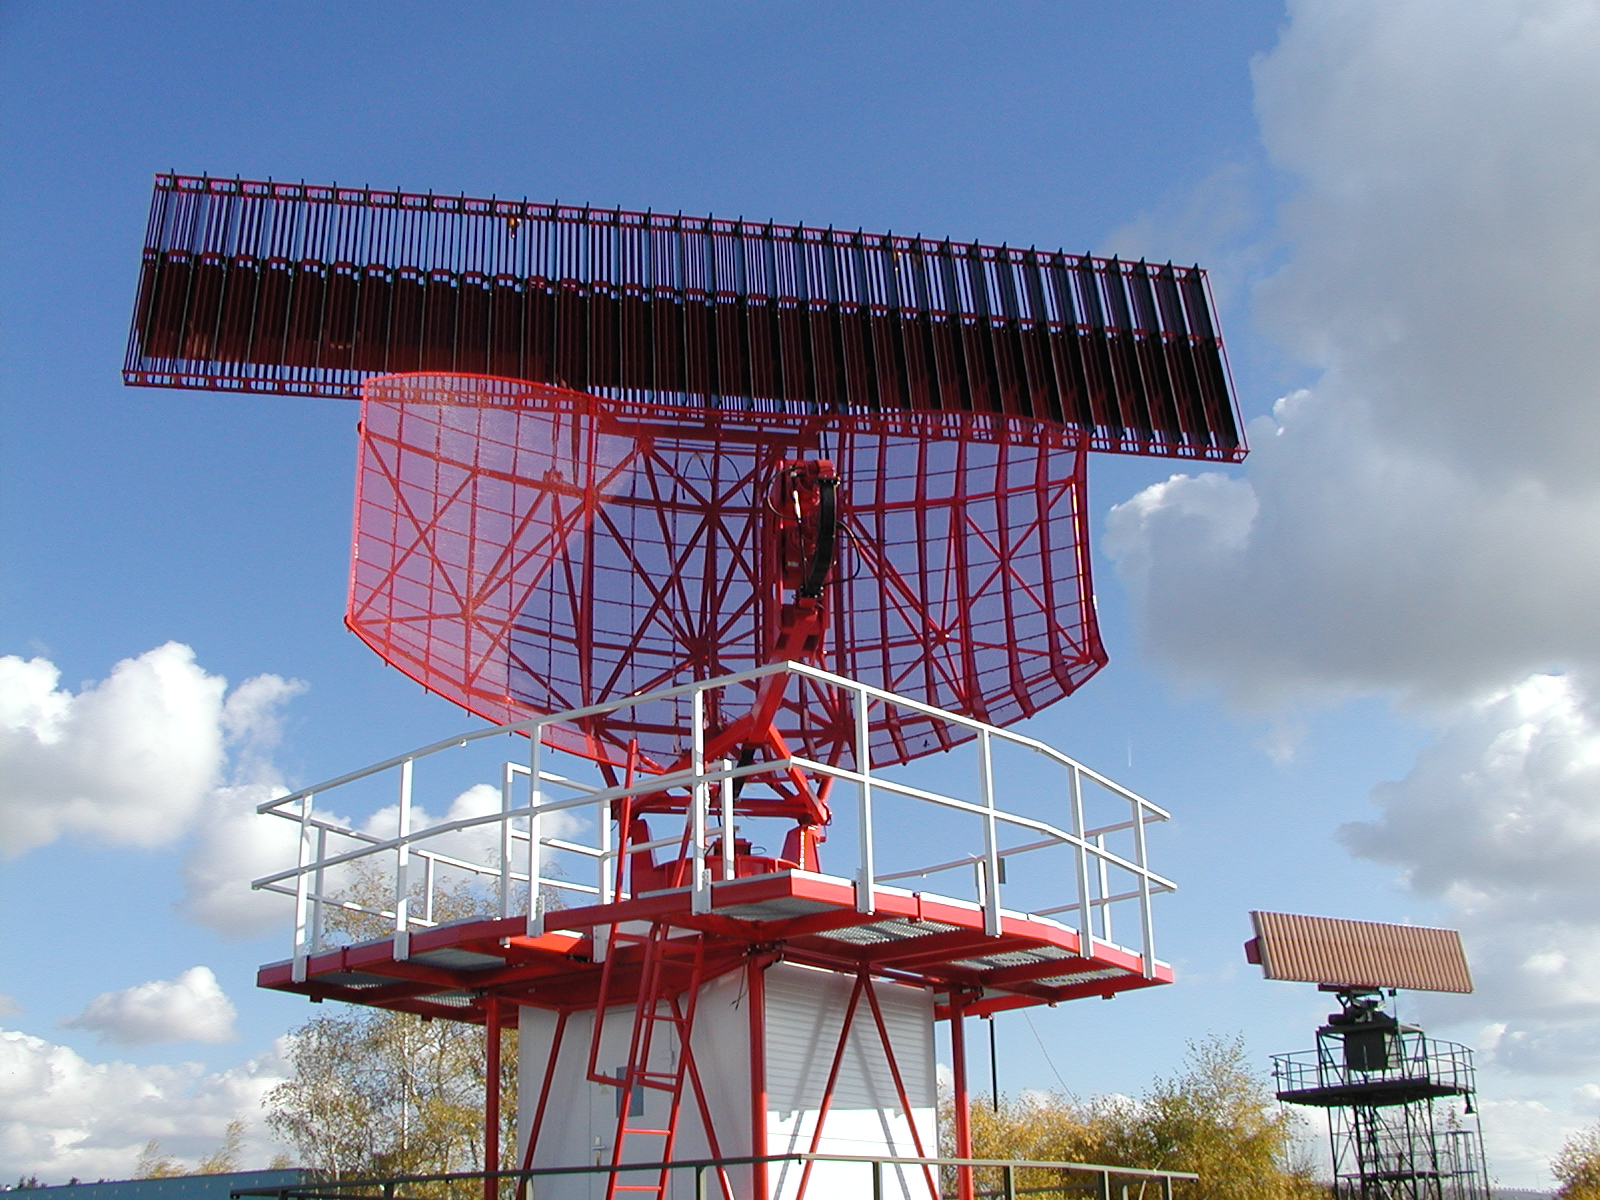
\includegraphics[width=0.9\textwidth]{Rotating_radar_antenna}
\caption{Rotating radar antenna}\label{fig:rotating_radar_antenna}
\end{minipage}\hfill
\begin{minipage}{0.3\textwidth}
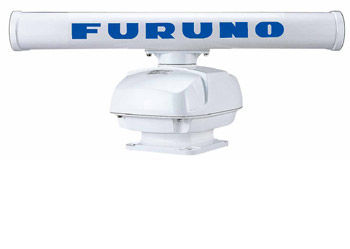
\includegraphics[width=0.9\textwidth]{Maritime_radar_antenna}
\caption{Maritime radar antenna}\label{fig:maritime_radar_antenna}
\end{minipage}
\end{figure}

\subsection{History}
The fist implementation of an instrument that were able to detect the presence of distance metallic objects by radio waves was done by Christian Hülsmeyer in 1904. His invention did not measure the distance to objects, but whether there was an object in the direction of the instrument. The radar as we know it today was introduced in the mid to late 1930's, with world war two triggering research to improve the still immature technology to be used in military applications. After the war, the technology matured and were put in use in several civil applications, where air traffic control, maritime safety and weather monitoring is the most common.

\subsection{Principles}
The electromagnetic waves that a radar emits travels at the speed of light in air and vacuum. It reflects back when there is a change in the density of the medium it is travelling through, which is what happens when radio waves hit targets. Electrically conductive materials tend to be good reflectors, since they have a very different atomic density than air. On the other hand, materials with poor conductivity, and also some magnetic materials, tend to absorb radio waves. Like light, there are many ways an incoming radio wave can be reflected, primarily dependent on the geometry of the target. A corner with angles less than 90\degsym{} will reflect the incoming radio waves directly back to the sender, and is a good thing on targets that want to be visible on a radar. This principle is the basis for radar reflectors commonly used to boost the radar signature on smaller vessels, see Figure~\ref{fig:corner_reflector}.
\begin{wrapfigure}{R}{0.3\textwidth}
\centering
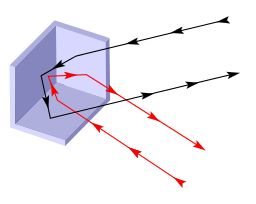
\includegraphics[width=0.25\textwidth]{Corner_reflector}
\caption{Corner reflector}\label{fig:corner_reflector}
\end{wrapfigure}
The opposite is used on targets that try to minimize their radar signature, and is the reason why stealth vessels and aircraft are tiled by flat areas. 
\begin{figure}
\centering
\begin{minipage}{0.3\textwidth}
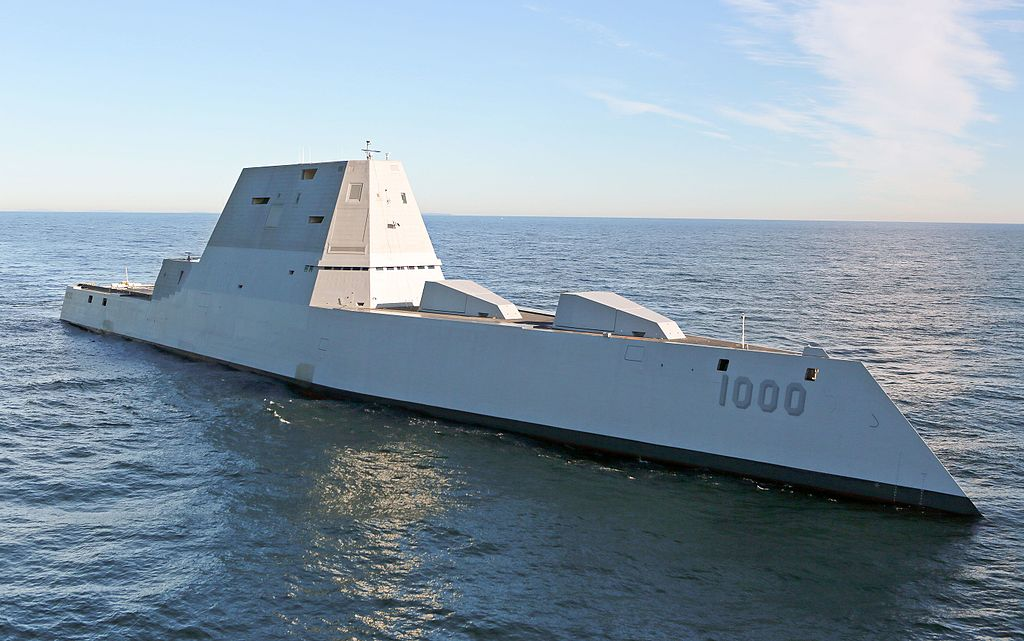
\includegraphics[width=0.9\textwidth]{USS_Zumwalt}
\caption{USS Zumwalt}\label{fig:uss_zumwalt}
\end{minipage}\hfill
\begin{minipage}{0.3\textwidth}
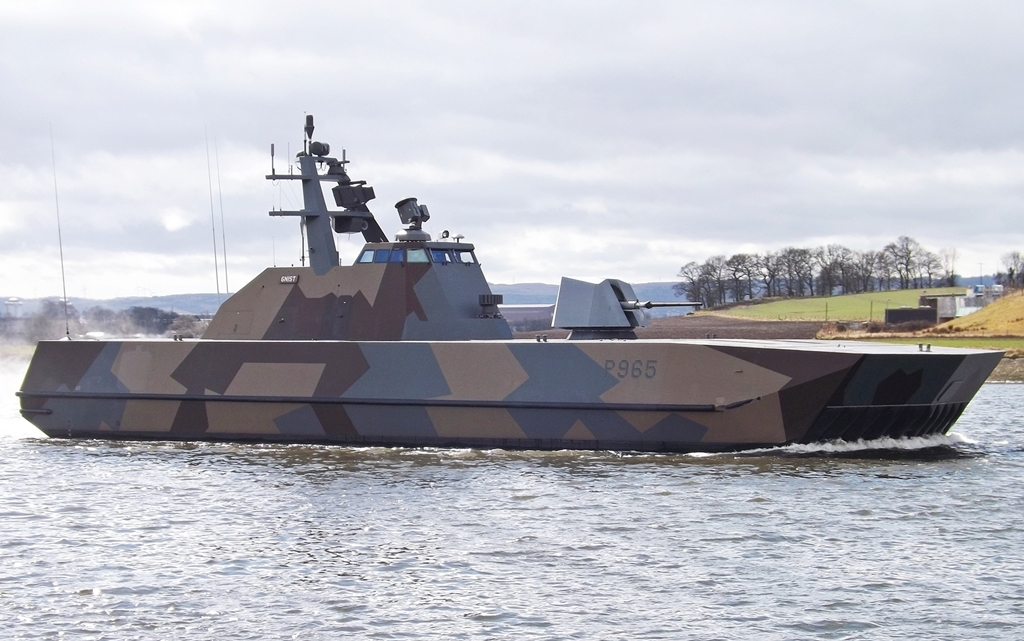
\includegraphics[width=0.9\textwidth]{KNM_Gnist}
\caption{KNM Gnist}\label{fig:knm_gnist}
\end{minipage}\hfill
\begin{minipage}{0.3\textwidth}
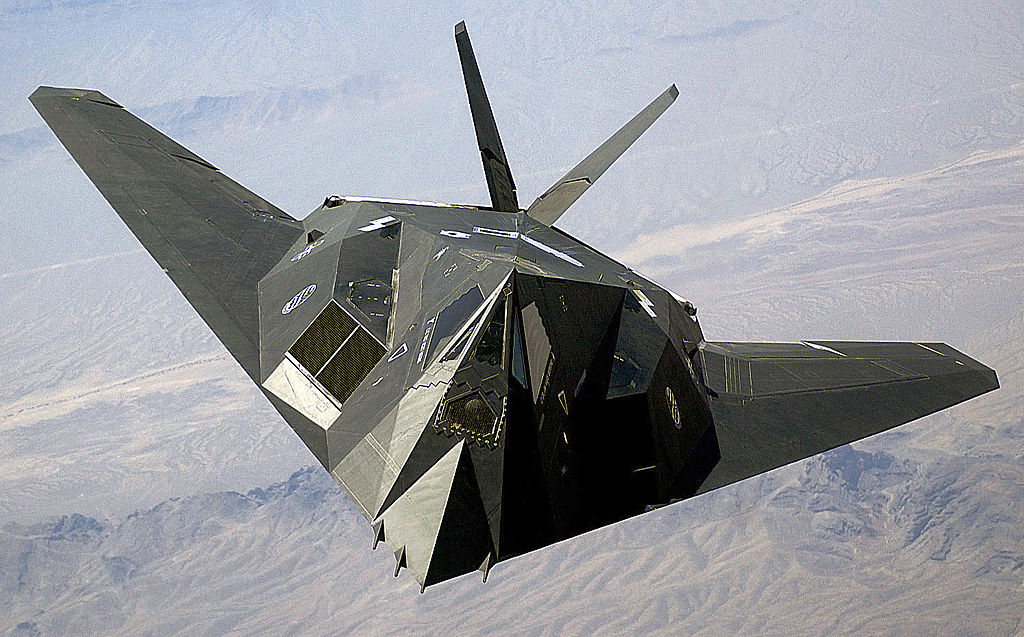
\includegraphics[width=0.9\textwidth]{Figures/F-117_Nighthawk}
\caption{F177 Nighthawk}\label{fig:f177_nighthawk}
\end{minipage}
\end{figure}

\section{AIS}
The \acrfull{ais} is a maritime safety and information system primarily designed for collision avoidance. \gls{ais} works by broadcasting messages on the \gls{vhf} band at irregular intervals with information on the vessels. \gls{ais} transceivers are required on international voyaging vessels over 300 \gls{gross_tonnage}, and on all passenger vessels. \gls{ais} signals are received at both vessels and shore stations for use in \gls{vts} stations, open tracking databases like \url{www.marinetraffic.com}, fleet-monitoring and search and rescue operations. Since the \gls{ais} messages contains position, course and speed, \gls{ais} tracks can be overlaid on a map in a chart plotter or on top of a radar image, giving the operator two sensors to verify each other.

\subsection{History}
\gls{ais} was designed and developed by technical committees in the \gls{imo}. Its objective was to enhance vessels safety and efficiency by increasing their ability to see and identify other vessels. The main motivation for adopting \gls{ais} was its independence of humans in operation, since it automatically identifies other vessels and displays the information on the navigational system on the bridge. It also enables automatic calculation of \gls{cpa} and time until \gls{cpa}, from which the navigation system could alarm the bridge of incoming traffic on dangerous course. This gives the navigator on the bridge more and better information for making decisions, but with the caveat that not all vessels have \gls{ais}. In the 2002 \gls{imo} \gls{solas} Agreement, it is required that vessels over 300 \gls{gross_tonnage} and all passenger vessels must be equipped with class A AIS transceivers. A simpler and cheaper \gls{ais} version named class B aimed at smaller vessels and yachts was published in 2006, followed by a large increase in the amount of non-commercial vessels equipped with \gls{ais}.

\subsection{Messages}
\gls{ais} broadcasts both static, dynamic and voyage information with varying intervals based on the vessels speed, status and on request from shore stations. Static, dynamic and voyage messages are listed in Table~\cref{tab:static-ais,tab:dynamic-ais,tab:voyage-ais}. When the \gls{ais} standard was developed, the peak traffic situations in the two most densely trafficked waterways, Singapore and Dover Straits, were used to calculate the update frequency for the AIS system. Based on these two locations and a desire to keep the number of reports per minute below 2000, the dynamic information report intervals for class A and B was set as in Table~\ref{tab:classA_reporting_intervals} and~\ref{tab:classB_reporting_intervals} respectively~\cite{IALA2004}. Static information is transmitted every 6 minutes, and on request from \gls{vts} stations. \gls{ais} transceivers are utilizing two reserved \gls{vhf} channels; AIS 1 --- 87B (161.975MHz) and AIS 2 --- 88B (162.025MHz) to improve robustness against interference. An important note is that \gls{ais} transceivers are alternating which channel they are transmitting on, which means that if a receiver is only listening on one channel, the effective update rate halves.

\begin{table}
	\begin{tabularx}{\textwidth}{XX}
	\toprule
	\multicolumn{2}{c}{Static AIS information} \\
	\midrule
	MMSI & Maritime Mobile Service Identity \\
	Call sign & Maritime radio (VHF) call sign \\
	Name & Name of vessel \\
	IMO Number & Vessel IMO number \\
	Length and beam & \\
	Location of positioning fixing antenna & \\
	Height over keel & \\
	\bottomrule
	\end{tabularx}~\caption{Static AIS information}\label{tab:static-ais}

	\vspace{0.5 cm}

	\begin{tabularx}{\textwidth}{XX}
	\toprule
	\multicolumn{2}{c}{Dynamic AIS information} \\
	\midrule
	Position & In WGS84 frame \\
	Position accuracy & Better or worse that 10 meter \\
	Position time stamp & UTC in whole seconds \\
	Course over ground (COG) & \\
	Speed over ground (SOG) & \\
	Heading & \\
	Navigational status & \\
	Rate of turn (ROT) & \\
	\bottomrule
	\end{tabularx}~\caption{Dynamic AIS information}\label{tab:dynamic-ais}

	\vspace{0.5 cm}

	\begin{tabularx}{\textwidth}{XX}
	\toprule
	\multicolumn{2}{c}{Voyage AIS information} \\
	\midrule
	Draught & Depth in water \\
	Hazardous cargo & Type \\
	Destination & Name of place \\
	Estimated time of arrival (ETA) & \\
	Route plan / waypoints & \\
	Number of persons on board & \\
	\bottomrule
	\end{tabularx}~\caption{Voyage AIS information}\label{tab:voyage-ais}
\end{table}

\begin{table}
	\centering
	\begin{tabularx}{0.8\textwidth}{b s}
	\toprule
	Vessels status & Reporting Interval \\
	\midrule
	Ship at anchor or moored \newline and not moving faster than 3 knots & 3 minutes \\
	Ship at anchor or moored \newline and moving faster than 3 knots & 10 seconds \\
	Ship 0--14 knots & 10 seconds \\
	Ship 0--14 knots and changing course & 3.3 seconds \\
	Ship 14--23 knots & 6 seconds \\
	Ship 14--23 knots and changing course & 2 seconds \\
	Ship > 23 knots & 2 seconds \\
	Ship > 23 knots and changing course & 2 seconds \\
	\bottomrule
	\end{tabularx}~\caption{Class A Reporting Intervals}\label{tab:classA_reporting_intervals}

	\vspace{0.5 cm}

	\begin{tabularx}{0.8\textwidth}{b s}
	\toprule
	Vessels status & Reporting Interval \\
	\midrule
	Ship < 2 knots & 3 minutes \\
	Ship 2--14 knots & 30 seconds \\
	Ship 14--23 knots & 15 seconds \\
	Ship > 23 knots & 5 seconds \\
	Search and Rescue aircraft & 10 seconds \\
	Aids to navigation & 3 minutes \\
	AIS base station & 10 seconds \\
	\bottomrule
	\end{tabularx}~\caption{Class B Reporting Intervals}\label{tab:classB_reporting_intervals}

\end{table}

\subsection{Class A}
Class A \gls{ais} transceivers are designed for \gls{sotdma} transmission, which is a way of reserving transmission time slot for the next broadcast. \gls{sotdma} is based on \gls{tdma}, with an extension allowing for self organizing of time slots compared to \glspl{tdma} dedicated timing manager. This effectively gives class A AIS transmissions priority over Class B equipment which may not have \gls{sotdma}. Class A transceivers are also required to have build-in display, minimum transmission power of 12.5W, ability to filter targets and communication interfaces like \gls{rs232} and \gls{nmea}.

\subsection{Class B}
Class B \gls{ais} transceivers are designed to be simpler and cheaper than Class A transceivers, which is accomplished through less strict requirements for hardware and operation. Class B \gls{ais} transmits at lower power, usually 2W and transmits at larger time intervals than Class A, see Table~\ref{tab:classB_reporting_intervals}. It is not required to have a build-in display and can use both \gls{cstdma} and \gls{sotdma} for transmission. \gls{cstdma} is a simpler approach to time division than \gls{sotdma} since it only listen for a single time slot to be unused before it transmits.

\section{Tracking}
\subsection{Overview}
Tracking, in this context, is the process of estimating the state of stationary and moving targets that are observed by a system without included association data. A key challenge is to know which measurements belong together over time, often referred to as the data association problem. An observation system can be a radar, sonar or any other sensor that, passively or actively, detects objects within an area or volume. Any observation system will be prone to noise, both in form of internal- and external noise from the environment. This noise will cause false measurements that the tracking system must take care of. These false measurements are often referred to as clutter.

In this work `tracking algorithm' will be used to describe the main logic in a tracking method or approach, while `tracking system' will be used on complete systems with everything around the main algorithm included. A tracking system can be defined as: \emph{A system that process consecutive measurements from one or more observation system and associates measurements from the same target into tracks with initialization of new tracks and termination of dead tracks}. A track is a sequence of states associated with a subset of all measurements from the observation systems. 

Tracking is a relative new field of study, driven by the military and aerospace industry and enabled by the development of microprocessors and computers from the 1960's. The applications ranges from sonar tracking of submarines from submarines and navy surface vessels to air traffic control and missile guidance. This historical background is likely the reason for most published papers using these types of applications as background for testing. In recent years, tracking people and vehicles from visual- and \gls{sar} imagery have also become a topic in the research community~\cite{Carthel2007,Carthel2007a,Coraluppi2000}. New applications areas like oceanography, autonomous vehicles and biomedical research have also found use of tracking~\cite{Wolf2010,Svec2014,Vo2015}.

There are several factors contributing to the challenge of good tracking; \gls{clutter}, lower than unity \gls{Pd}, multiple detections of the same vessel and wakes. \Gls{clutter} is a term for unwanted measurements or noise, which is inherent in every observation system. For a maritime radar, this can be caused by waves, rain, snow, birds or shore echo. A common assumption on clutter is to assume the amount being Poisson distributed, and spatially uniformly distributed. \gls{Pd} is a measure of how persistent the target is in the measurements, and will vary much between different types of targets, primarily dependent on their size, construction material and shape. Multiple detections of each target can occur when the target is large and have several distinct areas which reflects radar waves better than the rest of the vessel, for instance when the hull of a boat is made from fibreglass and the metal objects inside is reflecting. Wakes are reflection caused by the turbulent water behind a moving object, which can be a problem for both sonar and maritime- and air-radar.

\subsection{Single-target tracking}
The simplest approach to tracking is single-target tracking, where it is assumed that it is only one target in the surveillance area, and any other measurement is regarded as either extra measurements of the target or \gls{clutter}. 

\subsubsection*{\gls{nnf}}
The simplest single-target tracking algorithm is the \gls{nnf}, where the closest measurement is always selected~\cite{Bar-Shalom1998}. This approach is very vulnerable to clutter and dense multitarget scenarios.%, which is probably the reason its usage is very sparse. %Trenger kilder for eller mot denne påstanden 

\subsubsection*{\gls{pdaf}}
The most popular single-frame single-target tracking algorithm is \gls{pdaf}, which calculates probabilities of all target to measurement association for all measurement inside its gate. A gate is an ellipse (2D) or ellipsoid (3D) which outlines the confidence area / volume for a predicted state and covariance for a given confidence value. The state update is then based on a weighted sum of measurement innovations where the weightings are the probabilities for their respective innovations. \gls{pdaf}, like most tracking algorithms, assumes that at most one measurement is originating from the true target at each scan. It does not have a build-in initialization routine, and is dependent on an external initialization algorithm. One major drawback with \gls{pdaf} if using it to track multiple targets is its vulnerability to track \gls{coalescence}, which is when two tracks are merged into one `average' in between them~\cite{Blom2000}.

\subsection{Multitarget tracking}
A more generalized approach assuming that there can be any number of targets is called multitarget tracking, where the problem expands to jointly estimate several targets trajectories.

While a large number of tracking techniques have been developed, the three most used are \gls{jpdaf}, \gls{mht} and the \gls{rfs} paradigm~\cite{Vo2015}. Compared to \gls{mht} and \gls{jpdaf}, \gls{rfs} is a relatively new approach to tracking, and has not reached the same maturity as \gls{mht} and \gls{jpdaf}. \gls{mht} and \gls{jpdaf} also differs from \gls{rfs} in that they both do data association and filtering, whereas \gls{rfs} directly seeks both optimal and suboptimal estimates of the multitarget state~\cite{Vo2015}.

\subsubsection{JPDAF}
\gls{jpdaf} is a multitarget expansion of \gls{pdaf} which is a single-target tracking technique. \Gls{jpdaf} calculates joint posteriori association probabilities for every target in every scan. Each targets probability is a weighted sum over an exponential number of association hypotheses, where the weights are the key difference between \gls{pdaf} and \gls{jpdaf}. Like \gls{mht}, \gls{jpdaf} suffers from high computational cost. However, various approximations have been proposed, and an efficient implementation exist and is patented by QinetiQ~\cite{Horridge}. \Gls{jpdaf}, like its single target brother \gls{jpdaf} also suffer from track \gls{coalescence}. 

\subsubsection{MHT}
\gls{mht} is a decision logic which generates and maintains alternative hypotheses when new \glspl{measurement} are received within the gate. By making several possible hypotheses, the decision on which \gls{measurement} to choose can be propagated into the future when more information is available. MHT is a multi frame method, meaning it has the ability to utilize multiple scans to make better decisions. Each hypothesis is given a \gls{score} based on a likelihood ratio as a reflection of how well the measurement fits the model, which are accumulated to evaluate the combinations of consecutive \glspl{measurement}.

In contrast to the \gls{pdaf} and \gls{jpdaf} methods which suffers from track \gls{coalescence}~\cite{Fitzgerald1986,Blom2000}, \gls{mht} methods split when in doubt. The idea of using multiple hypotheses was first introduced by~\cite{Singer1974}, but the first complete algorithm was presented in~\cite{Reid1979}, where a \gls{homht} was developed. Following this, a \gls{tomht} was proposed in~\cite{Kurien1990} and the \gls{score} function for \gls{mht} was later deduced and discussed in~\cite{Bar-Shalom2007} since no explicit track-score function were given in~\cite{Kurien1990}. \gls{mht} is, in the same way as \gls{pdaf}/\gls{jpdaf}, developed under the main assumption that each target gives rise to maximally one \gls{measurement} (possibly zero if \gls{Pd} less than 1). The \gls{mht} approach to tracking and data association has been for a long time dismissed by many because of its computationally large cost. The dramatic increase in computational capability from the 1980's to the late 2010's has lead to a new spring for \gls{mht}, with an increasing interest for use in tracking system. In 2004 Blackman stated that \say{Multiple hypothesis tracking is generally accepted as the preferred method for solving the data association problem in modern multiple \gls{target} tracking system}~\cite{Blackman2004}. Already in 2001 did Blackman publish a demonstration that \gls{mht} is capable of real-time demands~\cite{Blackman2001}.

\gls{mht} comes in two variations, \gls{homht} and \gls{tomht}. They differ in their approach to arrange the measurements into hypotheses in that \gls{homht} builds hypotheses that are different ways of organizing the measurements into tracks, while \gls{tomht} maintains already existing tracks and a hypothesis is only a possible track for a single target and not all targets.
%TODO: Skriv videre her


\subsubsection{\gls{rfs}}
\Gls{rfs} is a family of Bayesian methods and filters that is based on representing a multitarget state as a finite set of single target states. 
%Alternativ 1
%By not having the multitarget states represented as a vector, the estimation error is more meaningful and mathematically consistent. This is because the vector representation is ordered, and thus the only meaningful way of representing the estimation error would be to minimize the estimation error over all permutations of states. This can be represented as distances between finite sets, and is a much more well defined and understood concept. 
%Alternativ 2
This leads to a more compact formulation of multitarget tracking, where the entire tracking problem can be expressed in terms of Bayes rule and the Chapman-Kolmogorov integral. This is known as the multitarget Bayes filter. 

The \gls{rfs} approach to multi sensor multitarget tracking was done by Mahler in 1994, which lay the foundation for the development of \gls{fisst}. One popular filter based on \gls{rfs} is the \gls{phd} filter. The \gls{phd} filter is an approximation of the multitarget Bayes filter derived by Mahler using \gls{fisst}~\cite{Vo2015}. The \gls{phd} filter normally estimates the number of targets and then selects the same numbers highest probable tracks. One large drawback with the \gls{phd} filter is its assumption that the predicted multitarget \gls{rfs} is Poisson distributed. This assumption is relaxed in the \gls{cphd} filter where the prior and predicted multitarget densities are independently and identically distributed cluster processes~\cite{Mahler2007}.

